%partie sur l'accélération matérielle


\subsection{Optimisation : utilisation de l'accélération matérielle avec OpenCL}

\subsubsection{L'accélération matérielle}

\paragraph{Introduction}
L'accélération matérielle d'une tâche informatique consiste à dédier une certaine partie d'une unité de calcul à une tâche spécifique. 
C'est ce qui est fait avec le traitement du son avec les cartes son, les cartes d'acquisition vidéo, ou encore l'affichage 3D avec les cartes graphiques.

\paragraph{Le GPU, ou Graphical Processing Unit}

Un ordinateur comporte un processeur, aussi appelé CPU, pour Central Processing Unit. Mais les ordinateurs modernes possèdent aussi des puces dédiées à l'affichage, qu'il soit 2D ou 3D. Ce sont les GPU.

Un CPU est une puce servant à effectuer rapidement des tâches non ou très peu parallélisées. Il comporte généralement plusieurs "coeurs", qui sont relativement peu nombreux (2 voire 4 pour des processeurs grand public). Il est possible d'effectuer des tâches simultanément sur tous ces coeurs, c'est ce qui est fait naturellement par le système d'exploitation, qui répartit les tâches entre les coeurs. Par exemple, lors de l'affichage d'une page web contenant une vidéo, le décodage de la vidéo peut être effectué par un coeur, tandis qu'un autre s'occupera de l'affichage de la page elle-même.

Un GPU, au contraire, est une puce fortement parallélisée, se trouvant sur les cartes graphiques, ou plus récemment dans une partie du CPU dédiée à l'affichage. Elle contient une multitude de petits "processeurs de flux" (plusieurs centaines pour des cartes graphiques modernes), effectuant tous la même tâche au même moment. Ceci est très utile pour l'affichage 3D, pour la compression vidéo, ou encore pour le traitement du son, grâce à des technologies telles que TrueAudio.

\begin{figure}[!h]
\centering
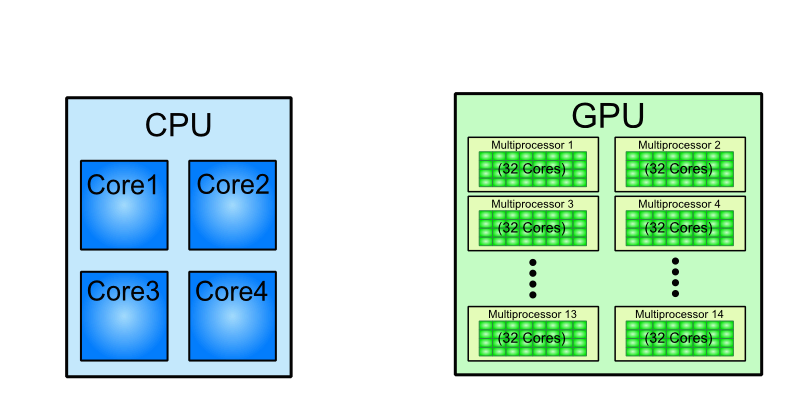
\includegraphics[scale=0.5]{images/cpugpu.png}
\caption{Comparaison entre les architectures CPU et GPU}
\label{cpugpu}
\end{figure}

\clearpage

\paragraph{Le calcul sur GPU}

Il est donc possible d'utiliser le GPU pour le traitement d'images, et donc pour notre transformation en ondelettes, puisqu'il s'agit de traiter une multitude de pixels de la même manière.
s
Les gains possibles sont importants, en effet, prenons l'exemple d'une image de 12 mégapixels (résolution classique pour un appareil photo moderne) et d'un GPU AMD Pitcairn (présent dans les cartes graphiques Radeon HD séries 7800) comportant 1024 processeurs de flux avec une fréquence de 1000MHz. Notre algorithme travaille sur des "blocs" de 4 pixels (comme vu plus haut) et fait environ une dizaine d'opérations de calcul sur ceux-ci, soit probablement un millier d'opérations élémentaires au niveau matériel environ.

Cela nous donne donc un temps de traitement théorique de l'ordre de $T = 12\cdot{}10^6 * 10^3 / 4 / 1024 / 1\cdot{}10^9 = 3\cdot{}10^{-3} s$. Ce qui est relativement faible en comparaison avec les temps obtenus avec un CPU. On peut donc bien parler "d'accélération" matérielle.

\subsubsection{Haar et OpenCL}

\paragraph{OpenCL}

OpenCL, pour Open Compute Language est un langage de programmation semblable au C, permettant de coder des tâches fortement parallélisées. Nous avons ici utilisé l'implémentation d'OpenCL en Python, appelée pyopencl. Le code OpenCL peut aussi bien être utilisé sur un CPU que sur un GPU, car tous les types de processeurs sont accessibles de la même manière au niveau de l'API elle-même, et sont appelés des "Workers".

\begin{figure}[!h]
\centering
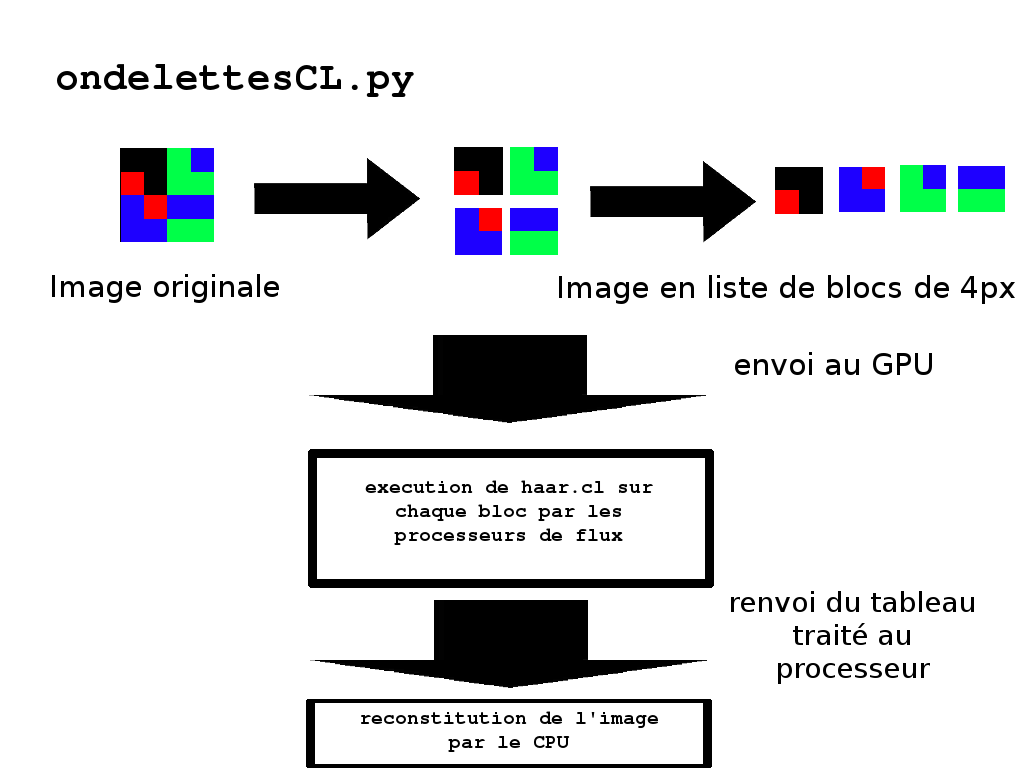
\includegraphics[scale=0.4]{images/haarcl.png}
\caption{Exécution de ondelettesCL.py}
\label{haarcl}
\end{figure}

\clearpage


\paragraph{L'implémentation de l'algorithme}

Les fichiers @ondelettesCL.py@ et @haar.cl@ peuvent être trouvés en annexe.

Implémenter un algorithme en pyopencl est simple, seule la partie à faire exécuter par le GPU est à coder dans un fichier différent, qui sera compilé à part lors du lancement du programme, puis envoyé à la carte graphique, qui l'exécutera ensuite quand il sera appelé par le programme principal. 

Le but est que chaque processeur de flux du GPU exécute la transformation montrée en section 7.5 sur un bloc de 4 pixels, avant de passer au suivant. On sépare donc l'image en ces blocs de 4 pixels, que l'ont met dans une grande liste, qui sera passée en argument au programme @haar.cl@.

Le fonctionnement du programme est représenté sur la figure 34.

\subsubsection{Performances réelles}

Le programme a été exécuté à l'aide d'un GPU AMD Radeon HD 7870, sur plusieurs images (voir annexes). Les temps d'exécution sont plus longs que les temps théoriques, ce qui est sans doute dû au temps de copie des données entre la mémoire RAM du système et celle du GPU.

\begin{figure}[!h]
\begin{center}
\begin{tabular}{|c|c|c|c|}
\hline
Image (résolution) & IMG1 (3 mégapixels)   & IMG2 (5 mégapixels)   &   IMG3 (12 mégapixels)   \\ 
\hline
Temps (secondes) & 0.057  & 0.079   &   0.122 \\
\hline
\end{tabular}
\end{center}
\caption{Temps d'exécution de haar.cl}
\label{tab7}
\end{figure}

Nous avons également surveillé l'activité du GPU lors du traitement à l'aide du logiciel MSI Afterburner. 

\begin{figure}[!h]
\centering
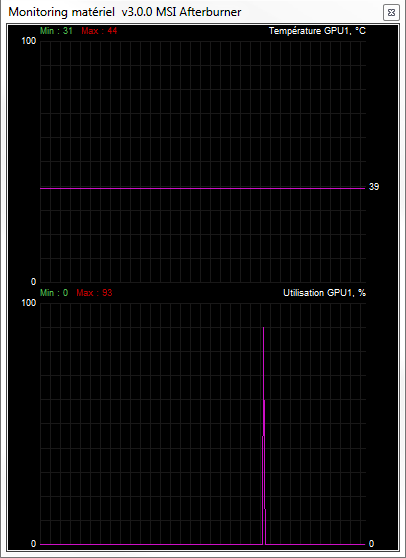
\includegraphics[scale=0.7]{images/monitor.png}
\caption{Graphique d'activité du GPU lors du traitement de l'image 3}
\label{afterburn}
\end{figure}

\clearpage
